

%Assumption of model, exponential decay
\subsection{Data Fit to Model of Damped Harmonic Oscillator}\label{sec:harmonic}
We tried to fit the data obtained from measurements of the \emph{normal} pendulum, the \emph{heavy} pendulum and the the pendulum with \emph{more air drag}. The result can be seen below in fig. \ref{fig:resultExp}.
%TODO write in how much more mass and how much more drag constant is affected.
\begin{figure}[htbp]
\centering
\begin{subfigure}{.45\textwidth}
	\centering
	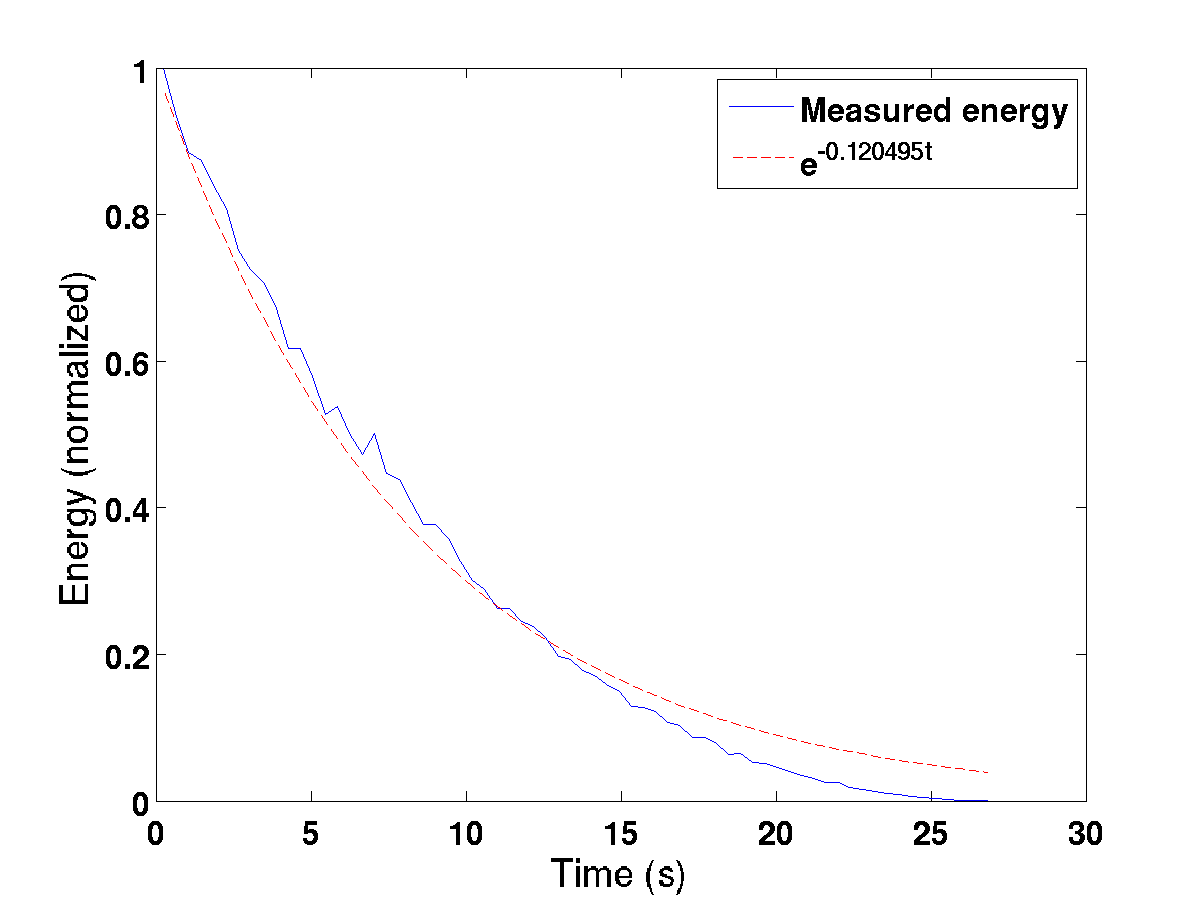
\includegraphics[width=\textwidth]{img/resultExpNormal}
	\caption{}
	\label{fig:resultExpNormal}
\end{subfigure}
\begin{subfigure}{.45\textwidth}
	\centering
	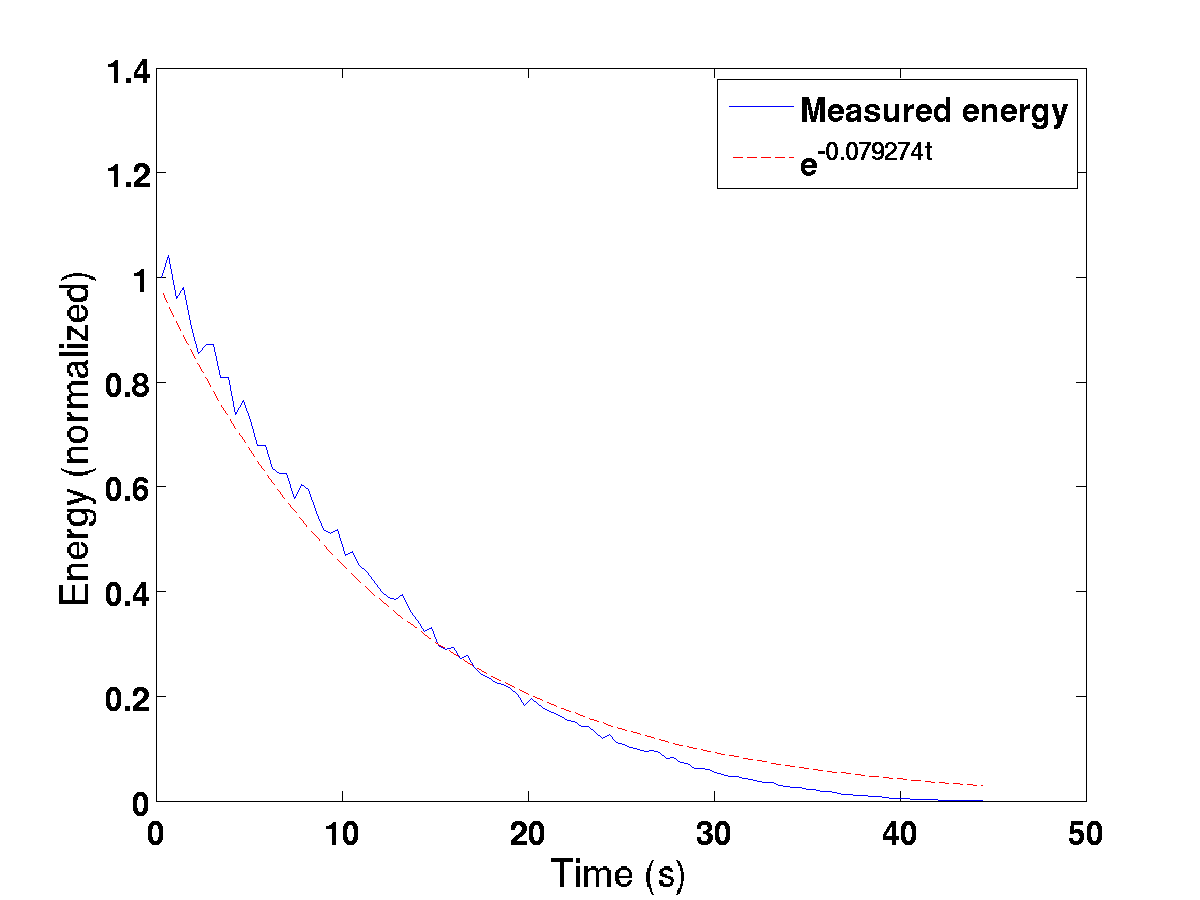
\includegraphics[width=\textwidth]{img/resultExpHeavy}
	\caption{}
	\label{fig:resultExpHeavy}
\end{subfigure}\\
\begin{subfigure}{.45\textwidth}
	\centering
	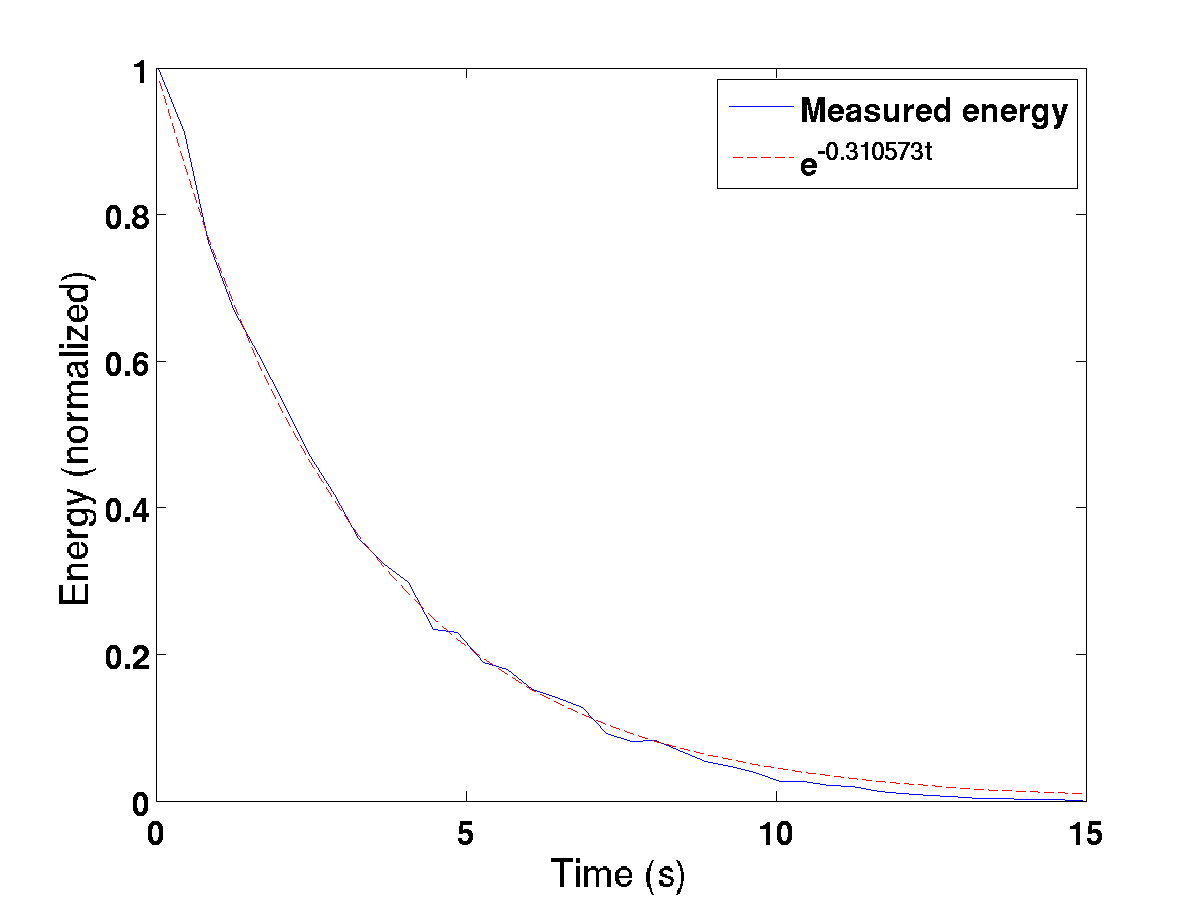
\includegraphics[width=\textwidth]{img/resultExpDraggy}
	\caption{}
	\label{fig:resultExpDraggy}
\end{subfigure}
\caption{Exponential decay fit to (a) normal weight and geometry of the  pendulum. (b) pendulum with added mass in the form of screw nuts. (c) pendulum with increased air drag due to changed geometry.}
\label{fig:resultExp}
\end{figure}

%TODO Tell us about what is interesting in the graph

\subsection{Data Fit to Novel Model Derived in Theory.}\label{sec:novel}
We then used eq. (\ref{eq:fullshort}) and fit the data obtained from measurements of the \emph{normal} pendulum, the \emph{heavy} pendulum and the the pendulum with \emph{more air drag}. The results can be seen in fig. \ref{fig:resultTan}.
%TODO write in how much more mass and how much more drag constant is affected.
%TODO Are these plots to small?
\begin{figure}[htbp]
\centering
\begin{subfigure}{.45\textwidth}
	\centering
	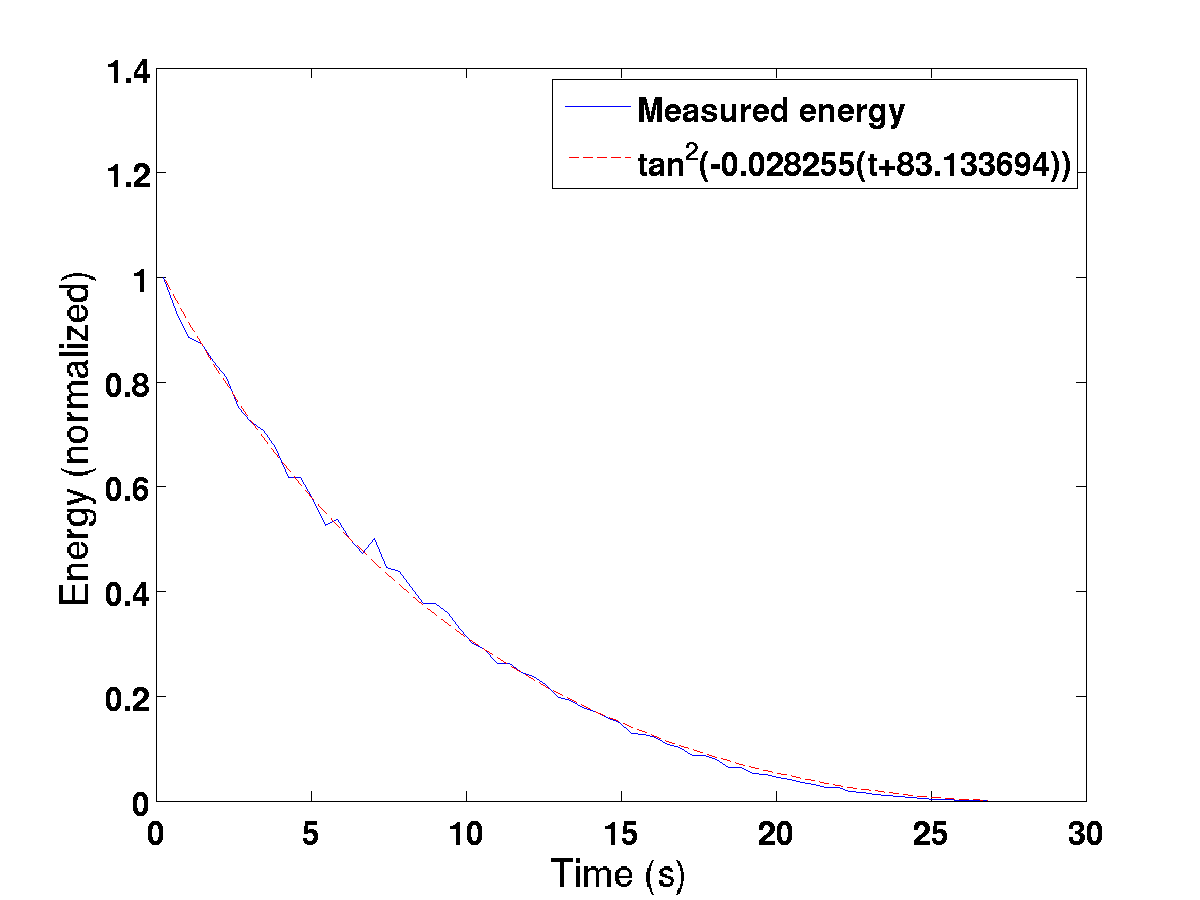
\includegraphics[width=\textwidth]{img/resultTanNormal}
	\caption{}
	\label{fig:resultTanNormal}
\end{subfigure}
\begin{subfigure}{.45\textwidth}
	\centering
	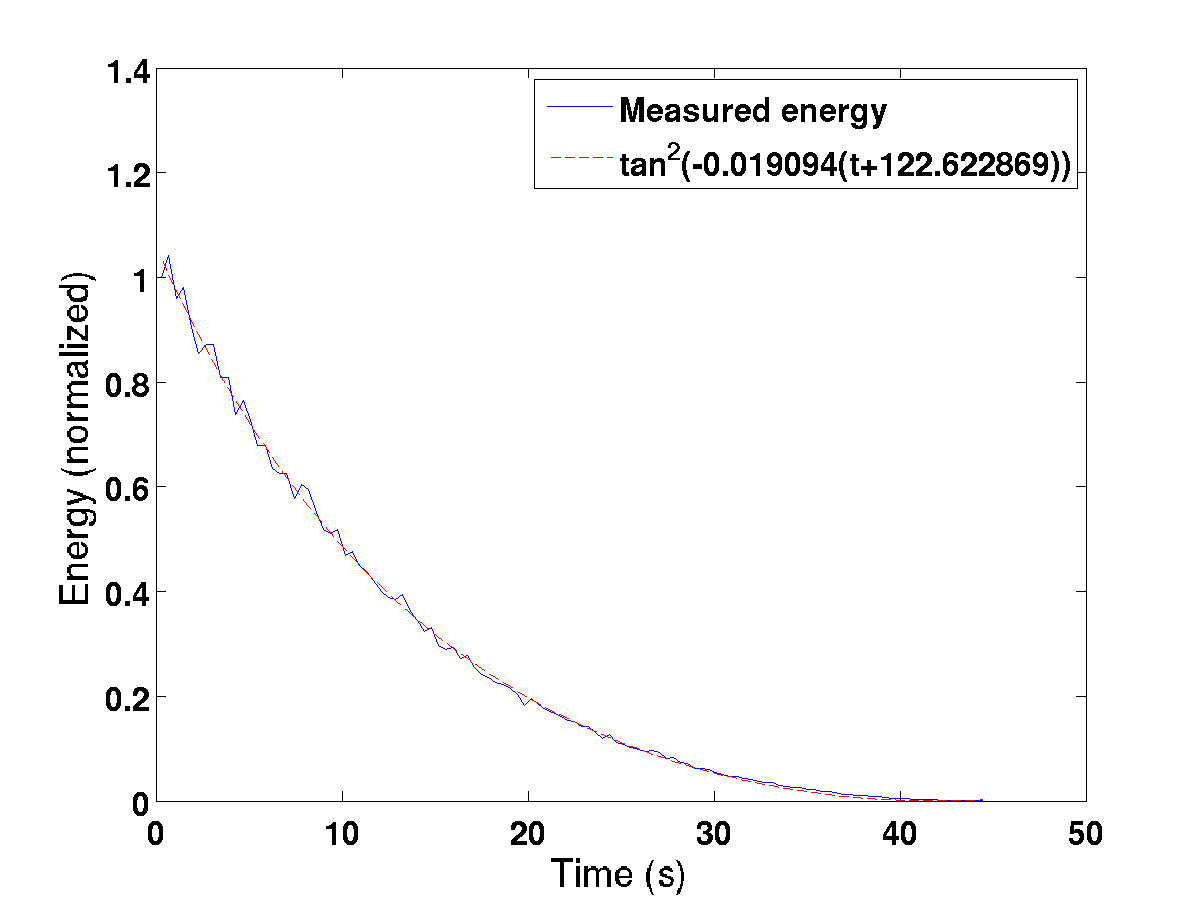
\includegraphics[width=\textwidth]{img/resultTanHeavy}
	\caption{}
	\label{fig:resultTanHeavy}
\end{subfigure}\\
\begin{subfigure}{.45\textwidth}
	\centering
	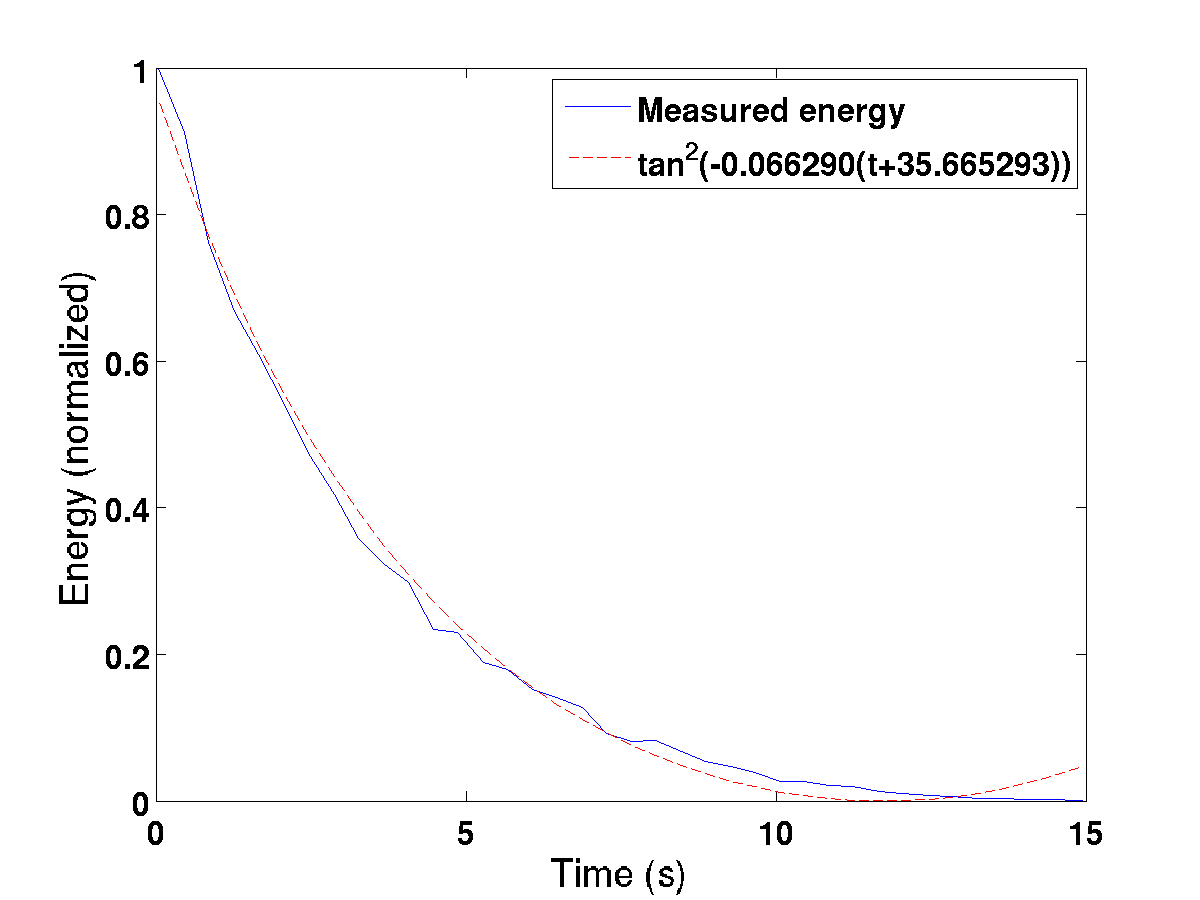
\includegraphics[width=\textwidth]{img/resultTanDraggy}
	\caption{}
	\label{fig:resultTanDraggy}
\end{subfigure}
\caption{Exponential decay fit to (a) normal weight and geometry of the  pendulum. (b) pendulum with added mass in the form of screw nuts. (c) pendulum with increased air drag due to changed geometry.}
\label{fig:resultTan}
\end{figure}

%TODO Tell us about what is interesting in the graph

\subsection{Analysis of Air Drag}\label{sec:airdrag}

Examining the pendulum with \emph{more air drag} we can assume that the friction due to the movement is neglectable. As in the theory suggested we can then apply fit function $ E(t)=4/\left(a t + b\right)^2$ (eq. (\ref{eq:air})) on the data. As already mentioned in section \ref{sec:experimental} three measurements with two different pieces of cardboard where made.  The results can be seen in fig. \ref{fig:resultSquare}.
\begin{figure}[htbp]
\centering
\begin{subfigure}{.45\textwidth}
	\centering
	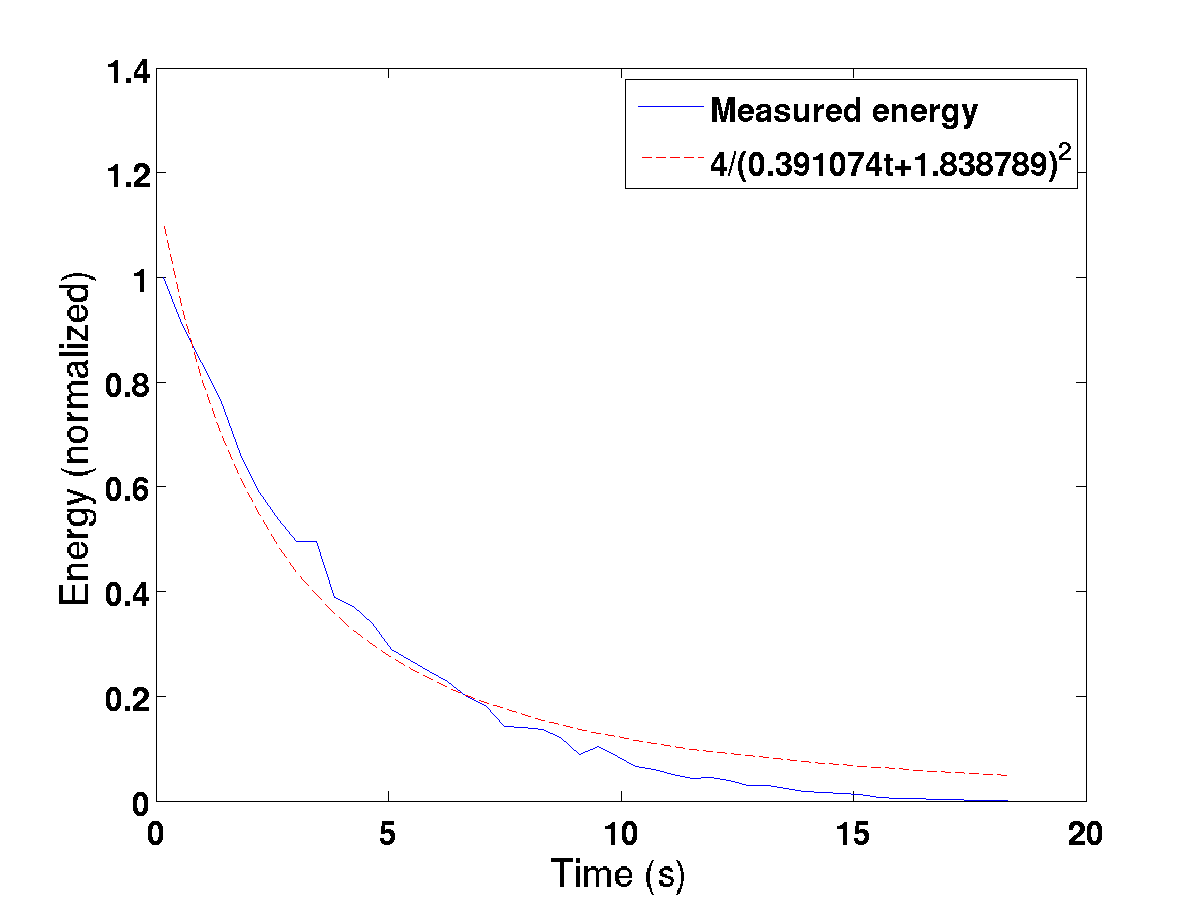
\includegraphics[width=\textwidth]{img/resultSquare1}
	\caption{}
	\label{fig:resultSquare1}
\end{subfigure}
\begin{subfigure}{.45\textwidth}
	\centering
	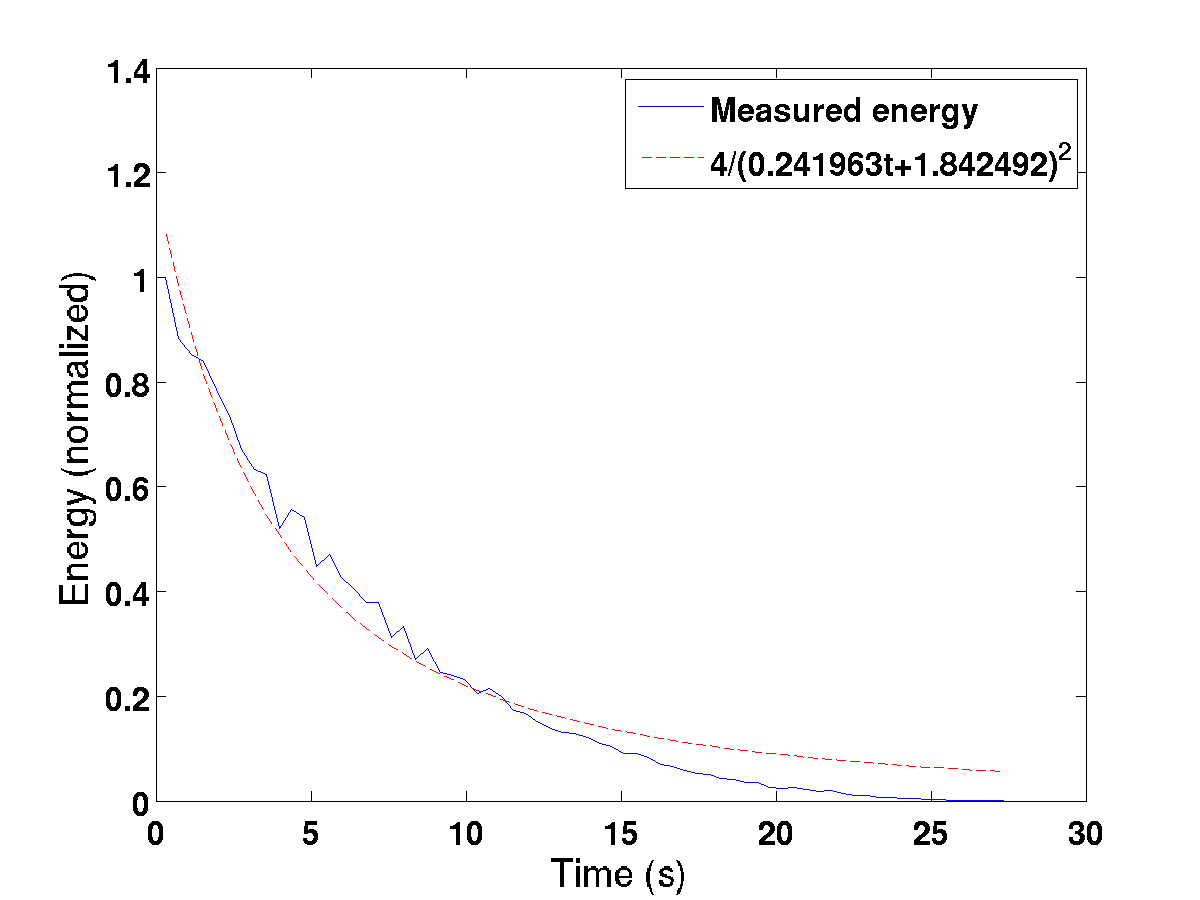
\includegraphics[width=\textwidth]{img/resultSquare2}
	\caption{}
	\label{fig:resultSquare2}
\end{subfigure}\\
\begin{subfigure}{.45\textwidth}
	\centering
	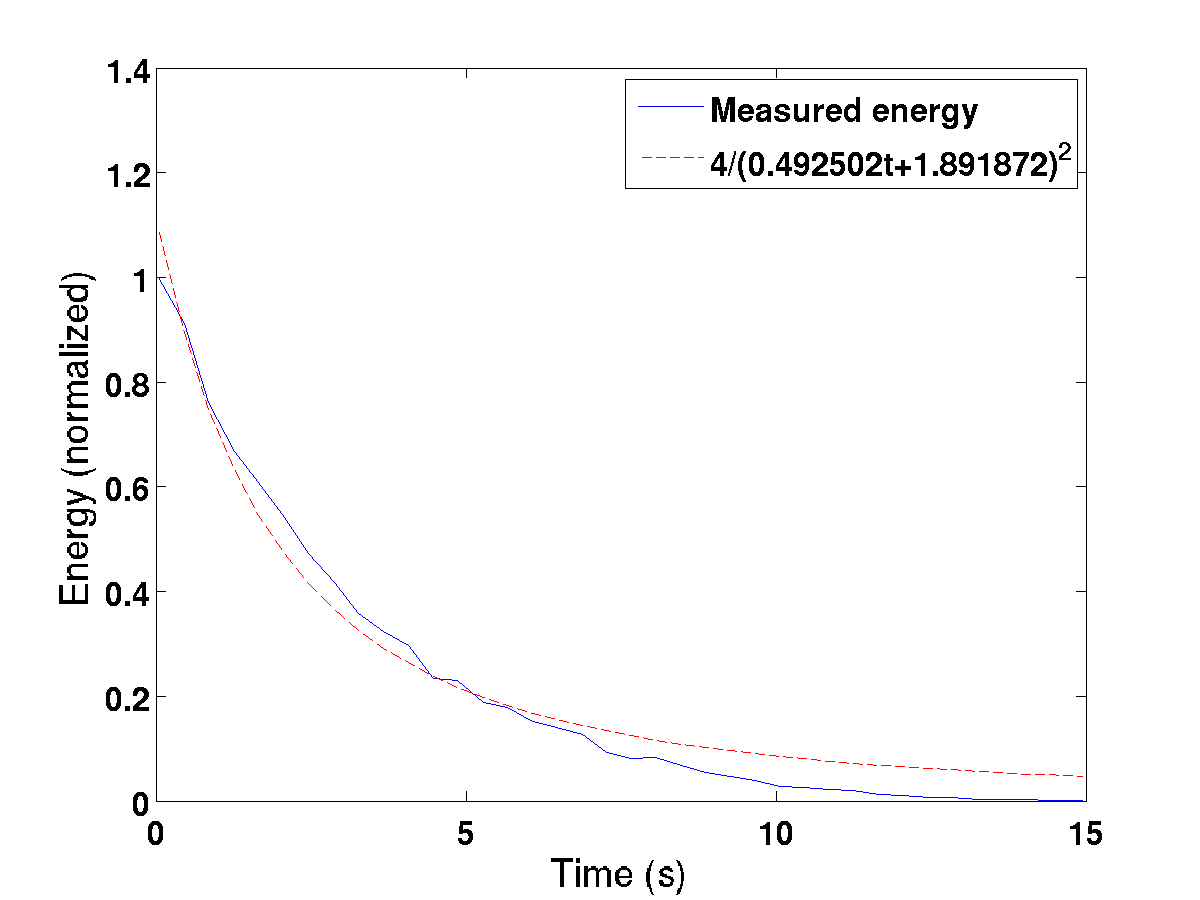
\includegraphics[width=\textwidth]{img/resultSquare1+2}
	\caption{}
	\label{fig:resultSquare1+2}
\end{subfigure}
\caption{Model fit to (a) geometry 1. (b) geometry 2. (c) geometry 1+2.}
\label{fig:resultSquare}
\end{figure}

From this figure we get
\begin{eqnarray}
a_{1+2} = 0.49\\
a_1 = 0.39 \\
a_2 =  0.24
\end{eqnarray}

As we can learn from the derivation of eq. (\ref{eq:taug}) in the theory it is not only important how large the cardboard is but also where it is fixed. So we have to consider which geometry was chosen during the measurement. This can be seen fig. \ref{fig:geometry}. 
\begin{figure}[htbp]
	\centering
	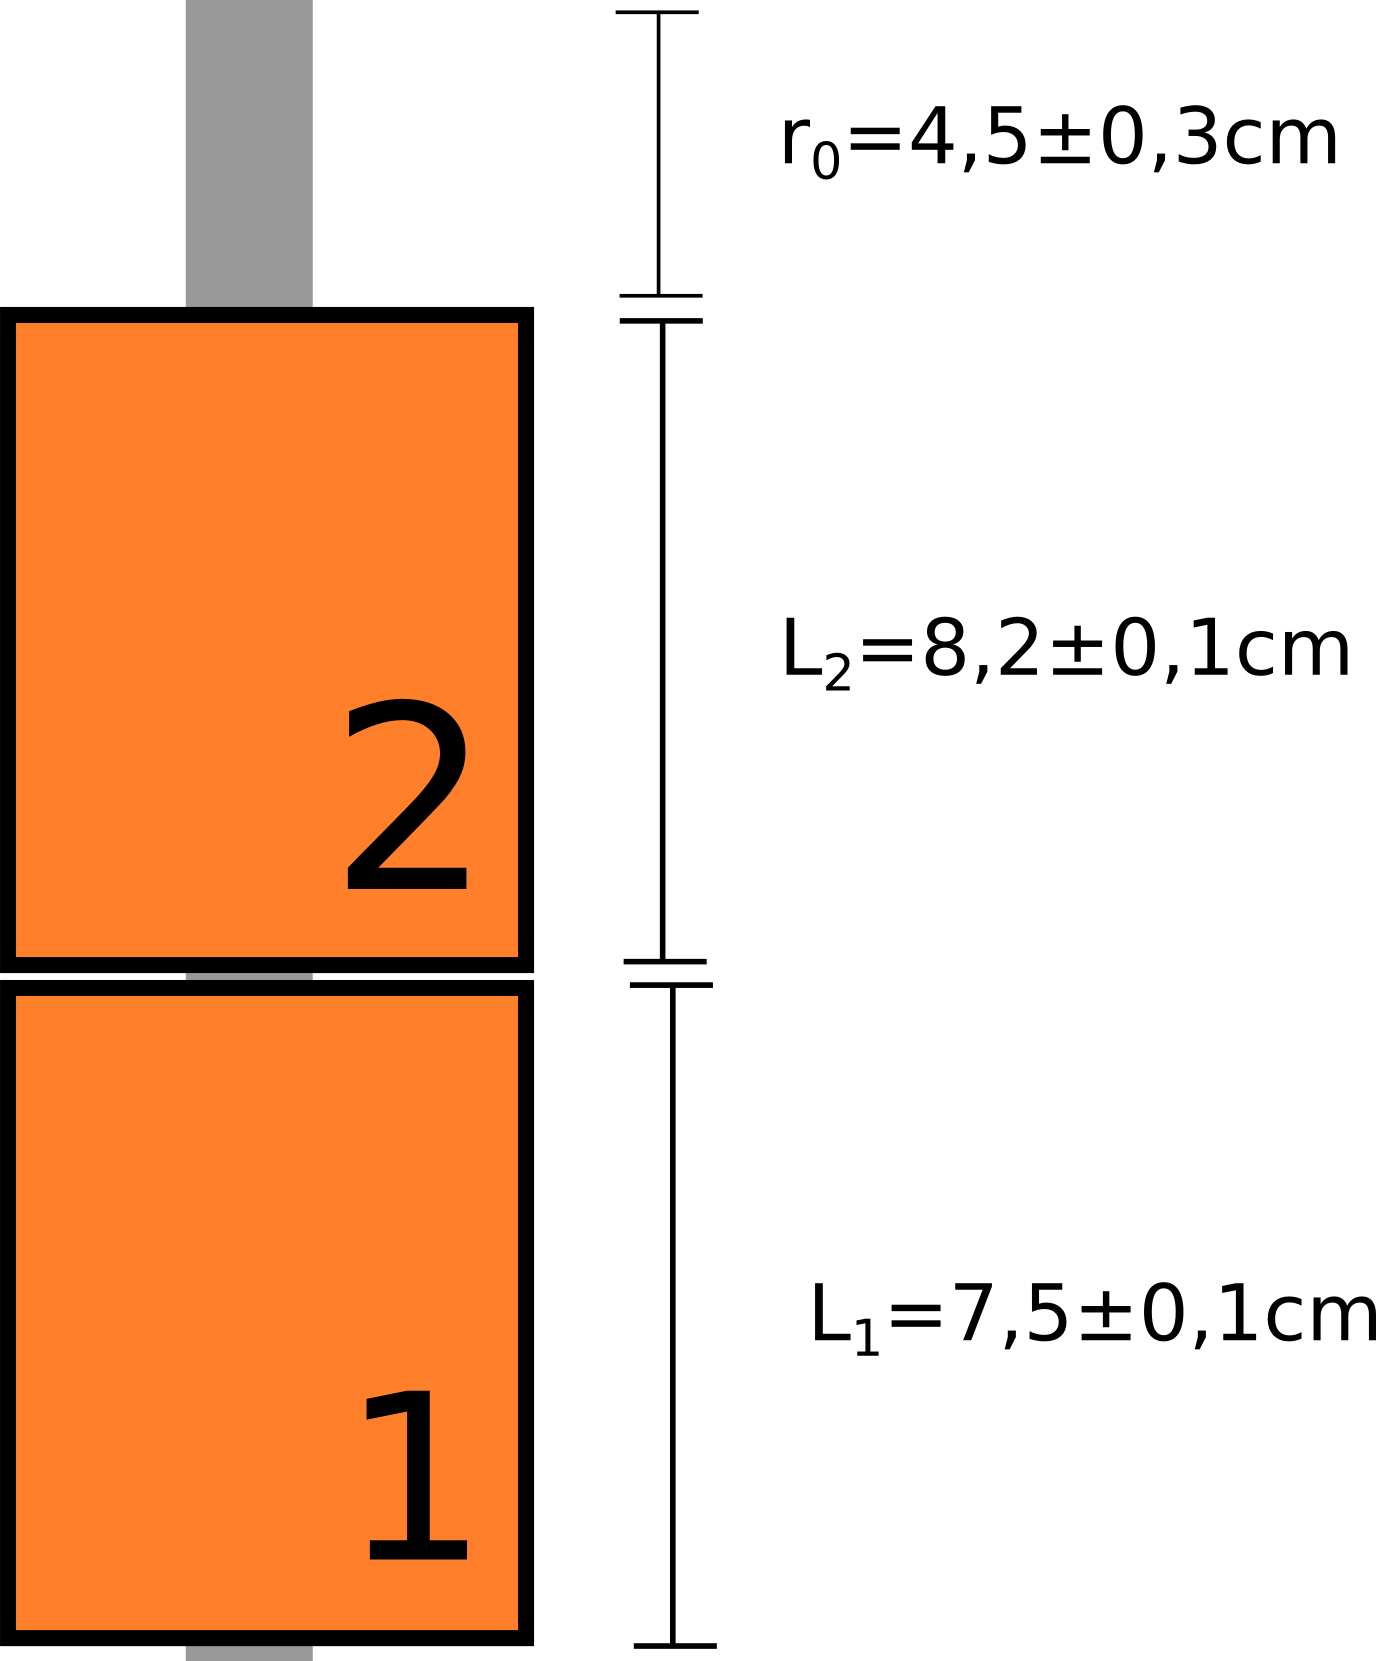
\includegraphics[width=0.5\textwidth]{img/draggeom}
	\caption{Illustration of how cardboard were added to the pendulum to increase air drag.}
	\label{fig:geometry}
\end{figure}
The position of the cardboards was never changed, the were just fixed and unfixed. The results confirm qualitatively the expectation from the theory on the first view: The largest damping is of course observed in the measurement with the biggest cross section (1+2). Since $v=\dot{\varphi}r$ we observe in measurement 1 a higher damping than in measurement 2. 

It is now interesting if we can compare the measurements also quantitatively with the theory. In equation  \ref{eq:taug} we would have to change the integration boundaries to consider the geometry in the right way. (Now we will just neglect the part of the pendulum that is not covered with cardboard.) So the theory suggests that:


\begin{eqnarray}
a_{1+2} \propto \left[ \left(r_0+L_2+L_1\right)^4-r_0^4\right]
a_1 \propto \left[ \left(r_0+L_2+L_1\right)^4-\left(r_0+L_2\right)^4\right]
a_2 \propto \left[ \left(r_0+L_2\right)^4-r_0^4\right]
\end{eqnarray}

Since no other parameters were modified the proportionality constants should be the same. So they can be determined by dividing the left-hand-sides by the right-hand-sides of the equations above. One gets we the values of fig ?? and the values form the fit-curves:
  
\begin{eqnarray}
C_{1+2} = 2,96 \cdot 10^{-6}
C_1 = 2,78 \cdot 10^{-6}
C_2 = 9,45 \cdot 10^{-6}
\end{eqnarray}

This does not look like the theory fits to the measured values. More about this in the discussion.

\subsection{calibration of distance between laser beams}\label{sec:calibration}
Through the use of simple trigonometry and fig. \ref{fig:calibration} we get the relation for the distance
$d$ between the beams at the point where the pendulum swings by to be
\begin{equation}
d = \frac{aB-A(D-B)}{D}
\end{equation}

\begin{figure}[htbp]
	\centering
	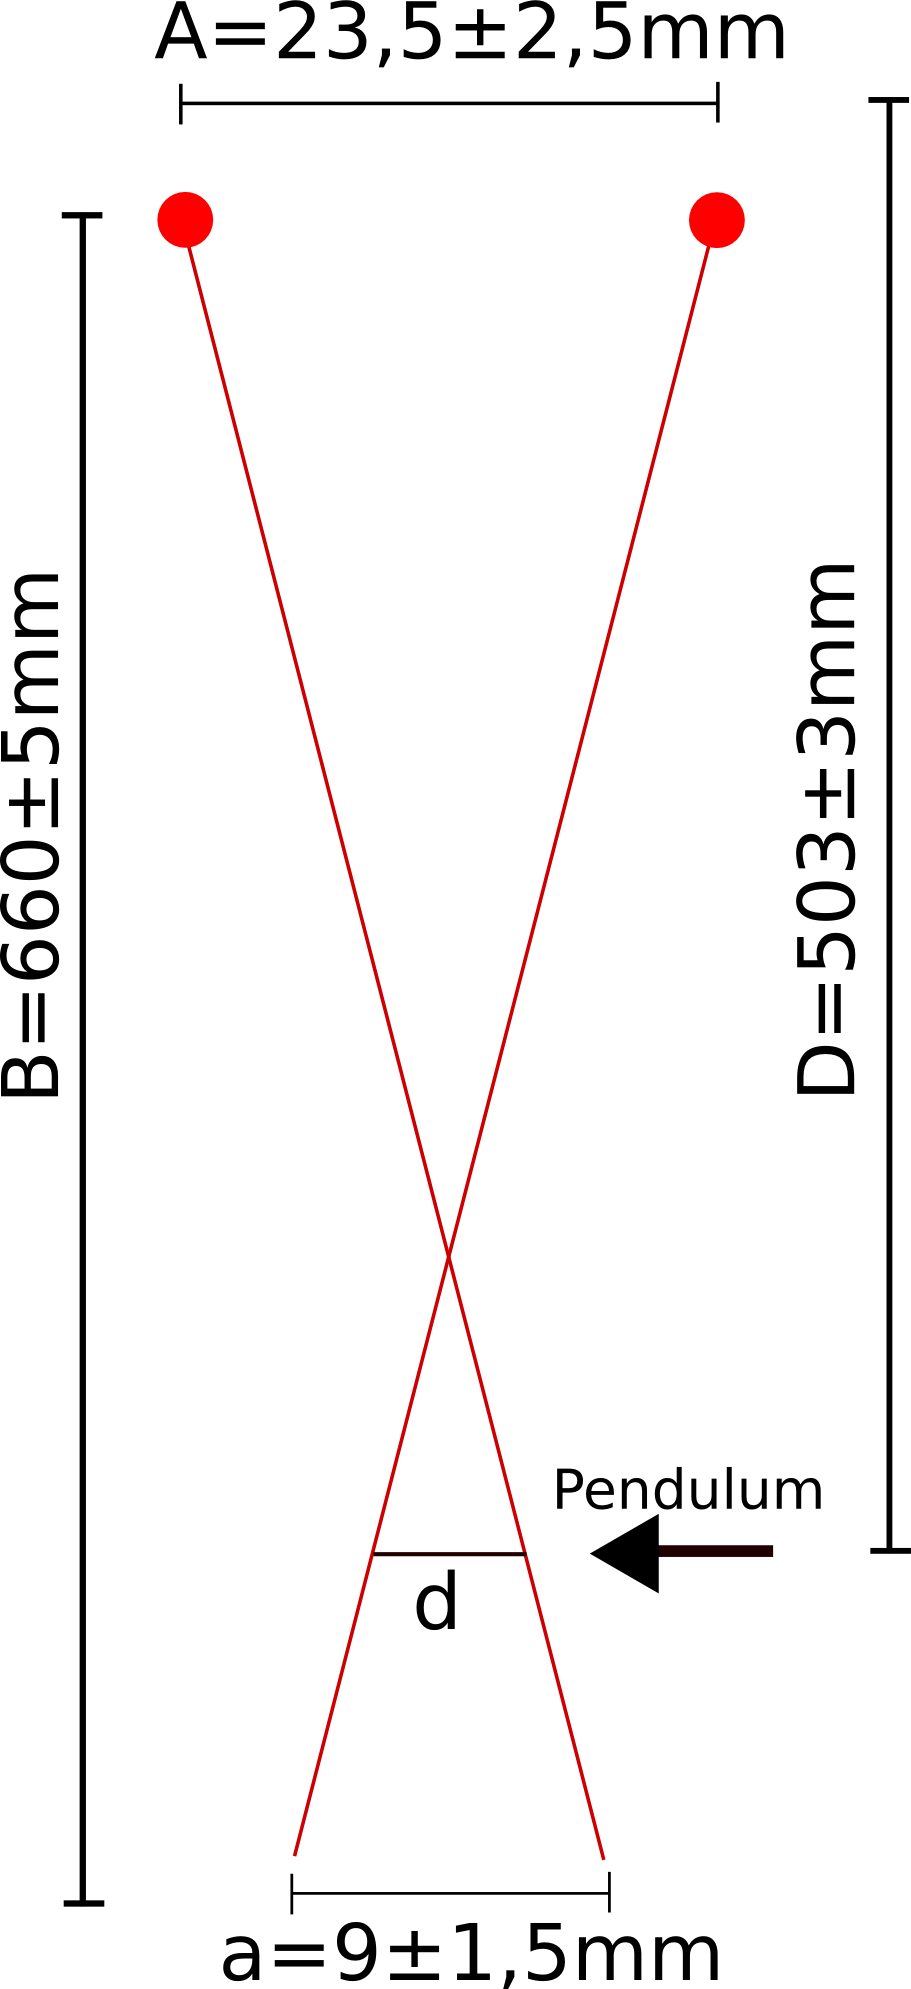
\includegraphics[width=0.5\textwidth]{img/calibration}
	\caption{$A$ is the distance between the photo diodes. $B$ is the distance between the beam splitter and the photo diodes. $D$ is the distance between the pendulum and the photo diodes. $a$ is distance between the laser beams where they originate from and $d$ is the unknown separation between the laser beams where the pendulum crosses.}
	\label{fig:calibration}
\end{figure}

For the measured distances and error estimates given in fig. \ref{fig:calibration} we get that
$d =  1.2689 \pm 1.3019 \rm{mm}$.
The error estimate was calculated using \emph{Gauss formula for uncertainty propagation}.


